\clearpage
\subsubsection{Eolian}
\begin{table}[h!]
\centering
\caption{Categorised GPR profile keywords for eolian environments. Geometry, reflectivity and continuity are shown in separate columns.}
\begin{tabular}{|p{5cm}|p{5cm}|p{5cm}|}
\hline
\textbf{Geometry / Structure} & \textbf{Continuity} & \textbf{Amplitude / Reflectivity} \\
\hline
Truncation & Semi-continuous & High reflectivity \\
Downlap & Discontinuous & Medium reflectivity \\
Oblique & Moderately continuous & Low reflectivity \\
Subparallel & Medium continuous & High amplitude \\
Horizontal subparallel & Continuous & Medium amplitude \\
Convex & &  \\
Concave & & High attenuation \\
Dipping & & \\
Multidirectional dipping & & \\
Horizontal & & \\
Sub-horizontal & & \\
Parallel & & \\
Tabular & & \\
Hummocky & & \\
Chaotic & & \\
Divergent & & \\
Diffraction hyperbolas & & \\
Tangential & & \\
Sigmoidal & & \\
Bounding surface & & \\
\hline
\end{tabular}
\label{tab:dune-coastal-keywords}
\end{table}

\begin{figure}[h!]
    \centering
    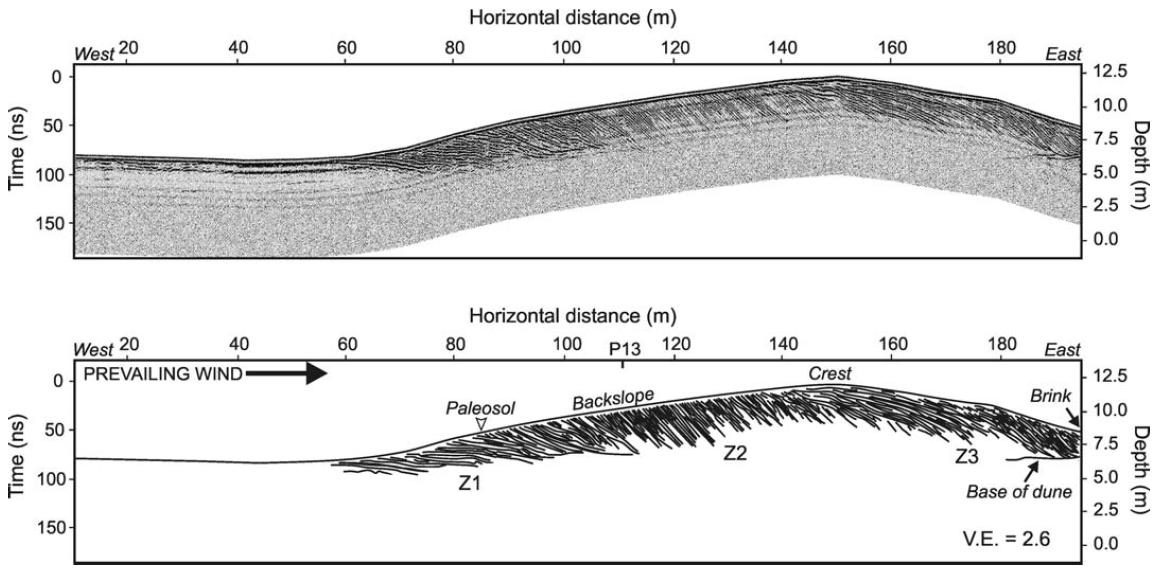
\includegraphics[width=0.9\linewidth]{Figures/0.2GPR/Hugenholtz_2007_1.png}
    \caption[Parabolic sand dune (2)]{Parabolic sand dune (2). \textbf{Keywords: } Truncation, downlap, oblique, subparallel, concave, dipping \citep{Hugenholtz2007}.}
    \label{fig:Hugenholtz2007-1}
\end{figure}

\begin{figure}[h!]
    \centering
    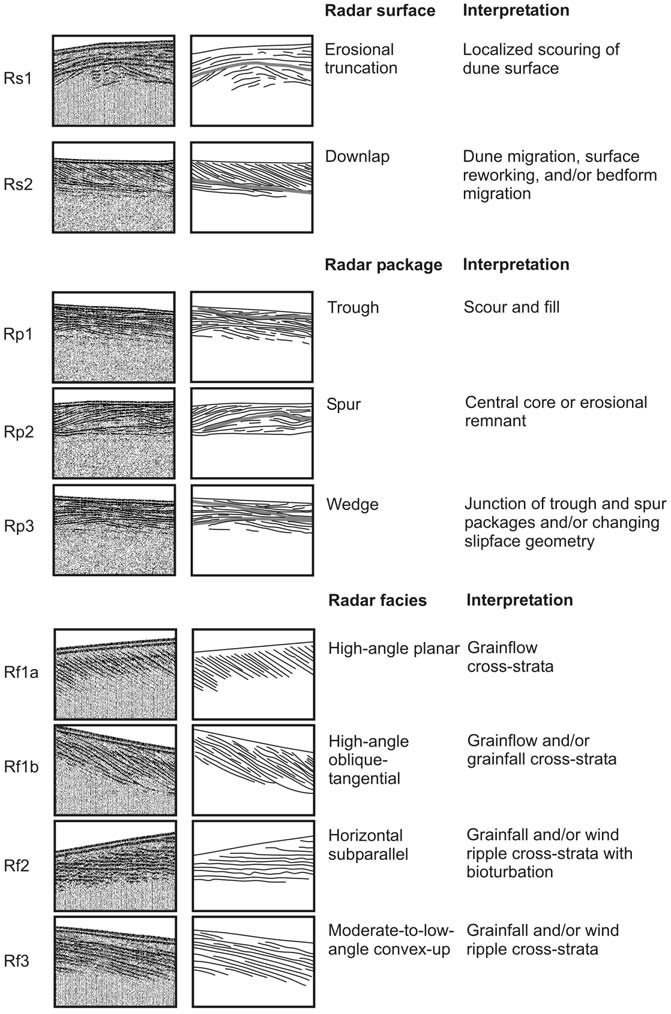
\includegraphics[width=0.9\linewidth]{Figures/0.2GPR/Hugenholtz2007_parabolicdunes.png}
    \caption[Parabolic sand dune (1).]{Parabolic sand dune (1). \textbf{Keywords: } Truncation, downlap, oblique, horizontal subparallel, convex, dipping \citep{Hugenholtz2007}.}
    \label{fig:Hugenholtz2007-4}
\end{figure}
\clearpage

\begin{figure}[h!]
    \centering
    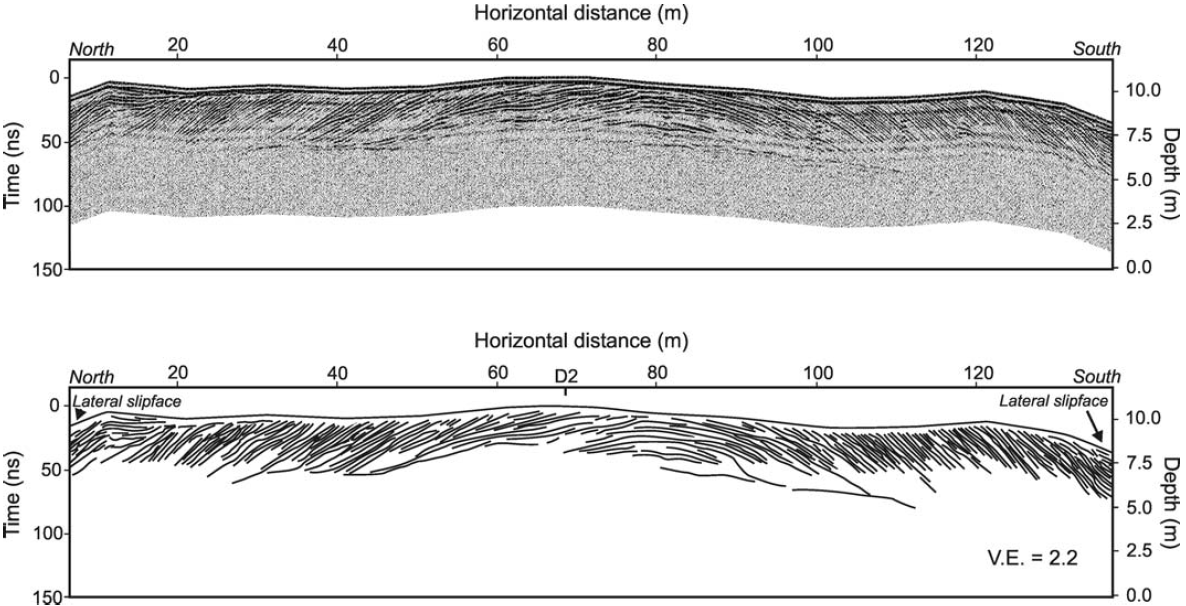
\includegraphics[width=0.9\linewidth]{Figures/0.2GPR/Hugenholtz_2007_3.png}
    \caption[Parabolic sand dune (3).]{Parabolic sand dune (3). \textbf{Keywords: } Truncation, downlap, oblique, subparallel, concave, multidirectional dipping \citep{Hugenholtz2007}.}
    \label{fig:Hugenholtz2007-3}
\end{figure}

\begin{figure}[h!]
    \centering
    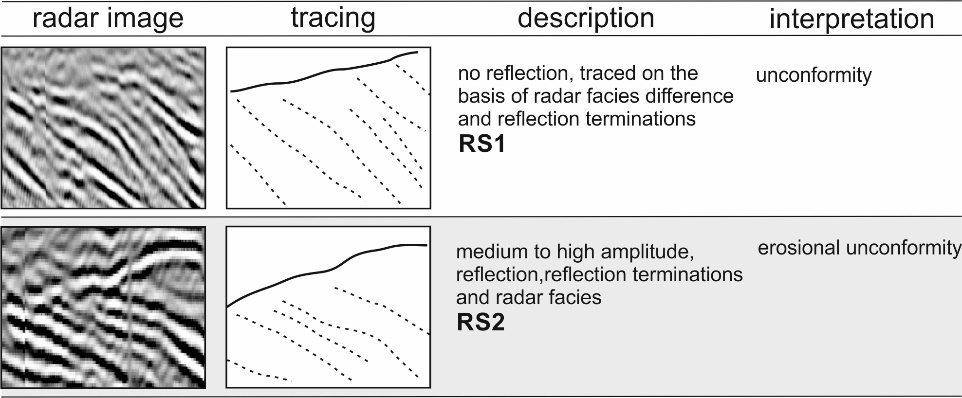
\includegraphics[width=0.9\linewidth]{Figures/0.2GPR/Ribolini2021_dunes_1.png}
    \caption[Coastal dunes (1).]{Coastal dunes (1). \textbf{Keywords: } Dipping, horizontal, convex, concave, chaotic, high attenuation, medium amplitude, high amplitude, moderately continuous, continuous, divergent, low amplitude, sub-horizontal, discontinuous, diffraction hyperbolas. \citep{Ribolini2021}.}
    \label{fig:Ribolini2021-1}
\end{figure}


\begin{figure}[h!]
    \centering
    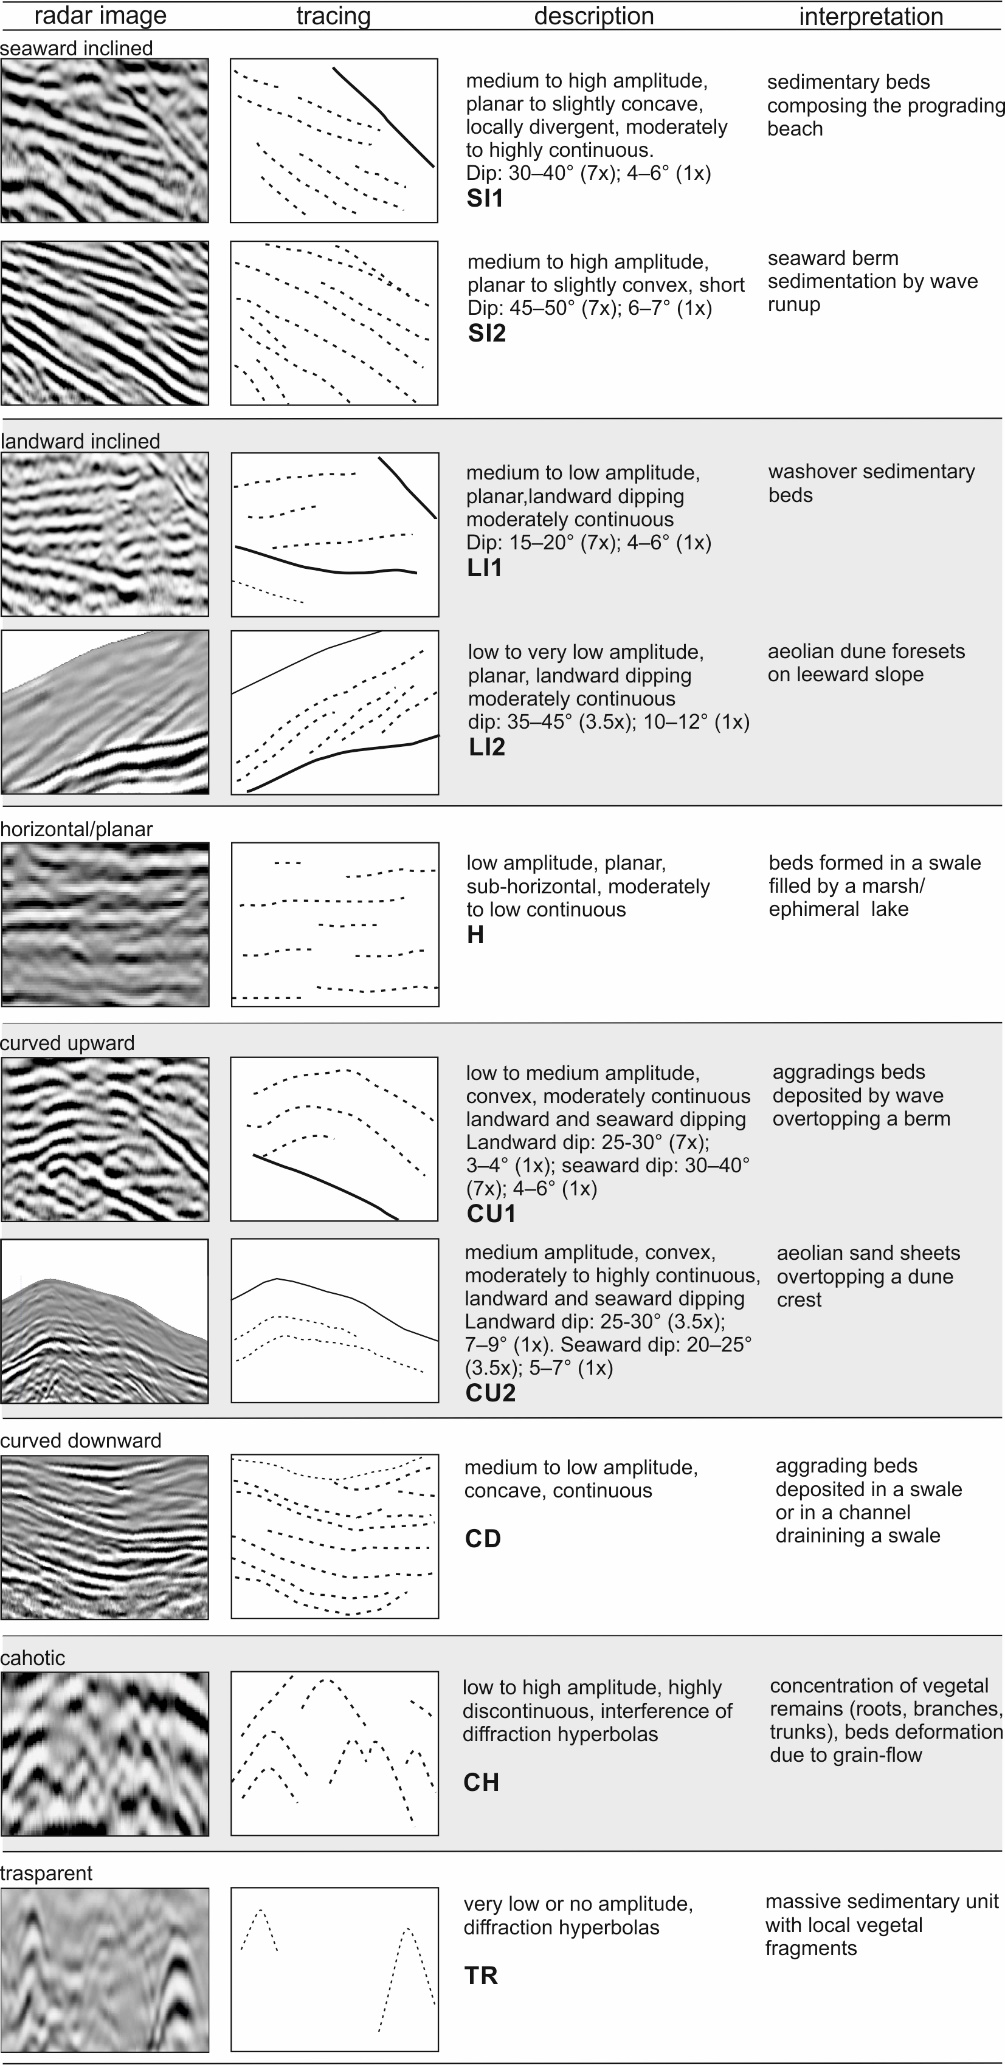
\includegraphics[width=0.75\linewidth]{Figures/0.2GPR/Ribolini2021_dunes_2.png}
    \caption[Coastal dunes (2).]{Coastal dunes (2).\textbf{Keywords: } Medium amplitude, high amplitude, concave, medium continuous, low amplitude, sub-horizontal, discontinuous, diffraction hyperbolas, high attenuation \citep{Ribolini2021}.}
    \label{fig:Ribolini2021-2}
\end{figure}


\clearpage
\begin{landscape}
    \begin{figure}[h!]
    \centering
    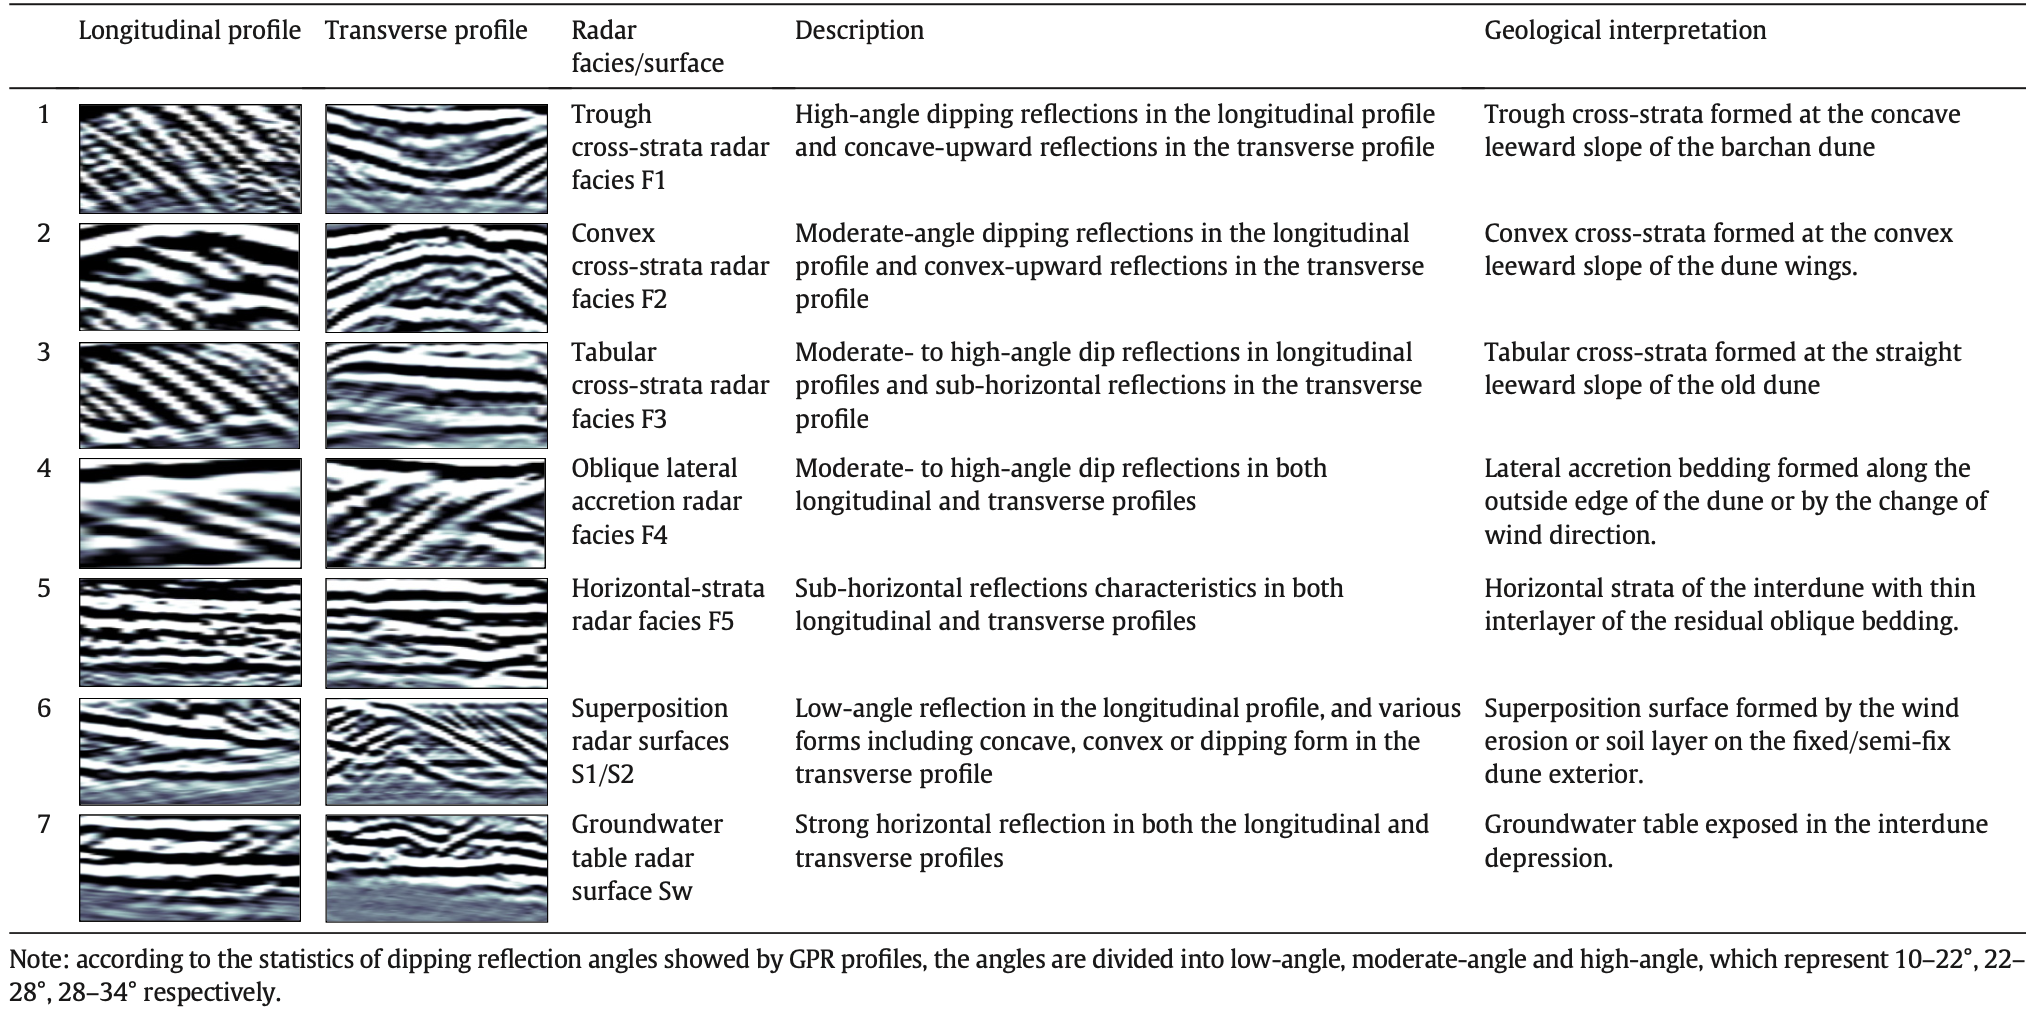
\includegraphics[width=0.8\linewidth]{Figures/0.2GPR/Fu_2019_dunes_1.png}
    \caption[Barchan dune (1).]{Barchan dune (1). \textbf{Keywords: } Dipping, concave, convex, sub-horizontal, tabular, horizontal, high reflectivity, medium reflectivity, semi-continuous, discontinuous \citep{Fu2024}.}
    \label{fig:Fu2019-1}
\end{figure}
\end{landscape}

\begin{figure}[h!]
    \centering
    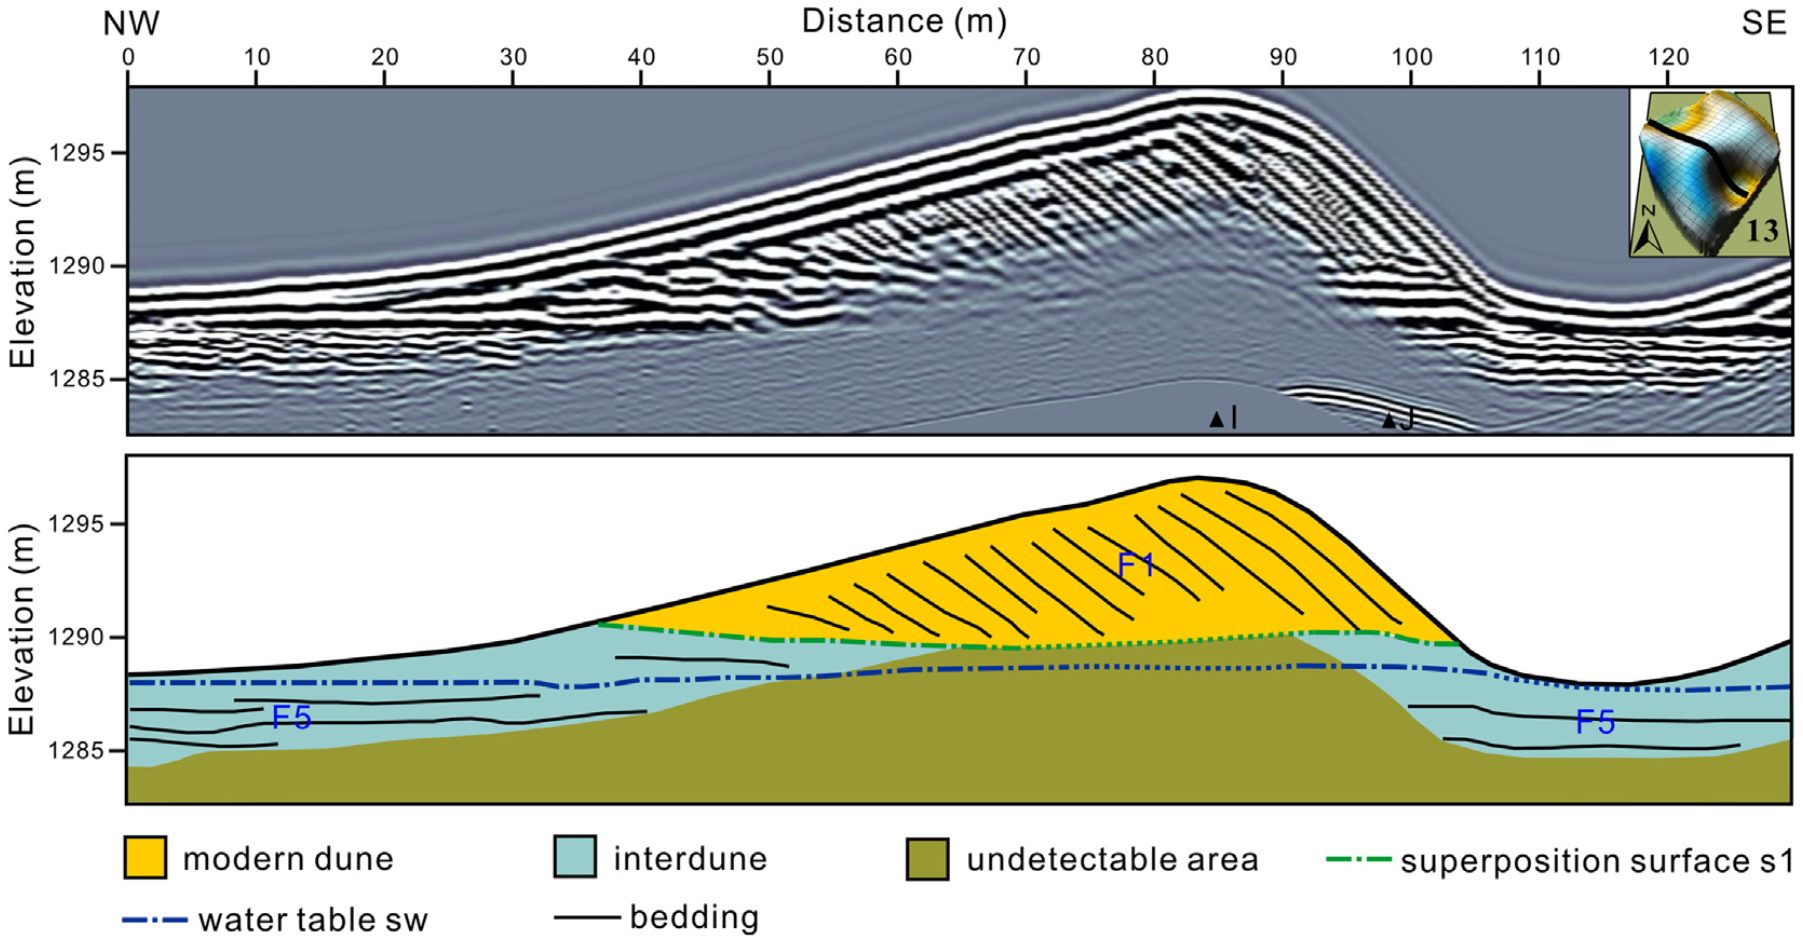
\includegraphics[width=0.9\linewidth]{Figures/0.2GPR/Fu_2019_dunes_2.png}
    \caption[Barchan dune (2).]{Barchan dune (2). \textbf{Keywords: } Horizontal, dipping, high reflectivity, low reflectivity, parallel, semi-continuous \citep{Fu2024}.}
    \label{fig:Fu2019-2}
\end{figure}

\begin{figure}[h!]
    \centering
    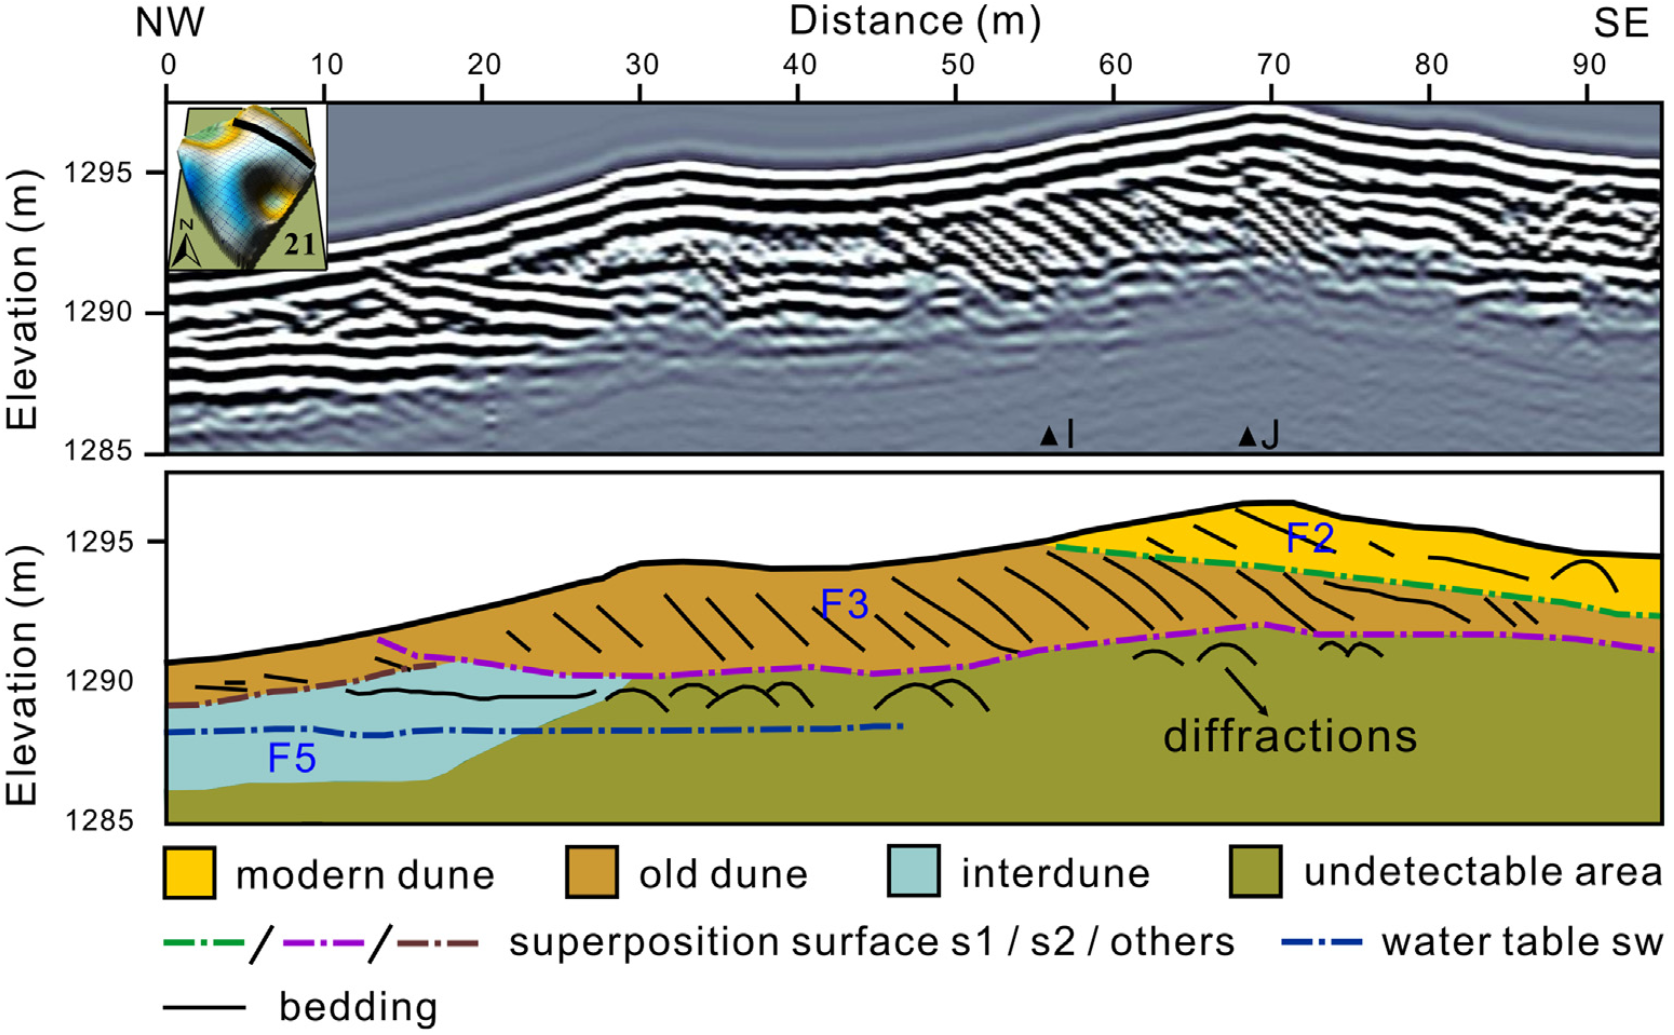
\includegraphics[width=0.9\linewidth]{Figures/0.2GPR/Fu_2019_dunes_4.png}
    \caption[Barchan dune (2).]{Barchan dune (2). \textbf{Keywords: } Parallel, semi-horizontal, semi-continuous, dipping, hummocky, diffraction hyperbola, high reflectivity, low reflectivity \citep{Fu2024}.}
    \label{fig:Fu2019-4}
\end{figure}

\begin{figure}[h!]
    \centering
    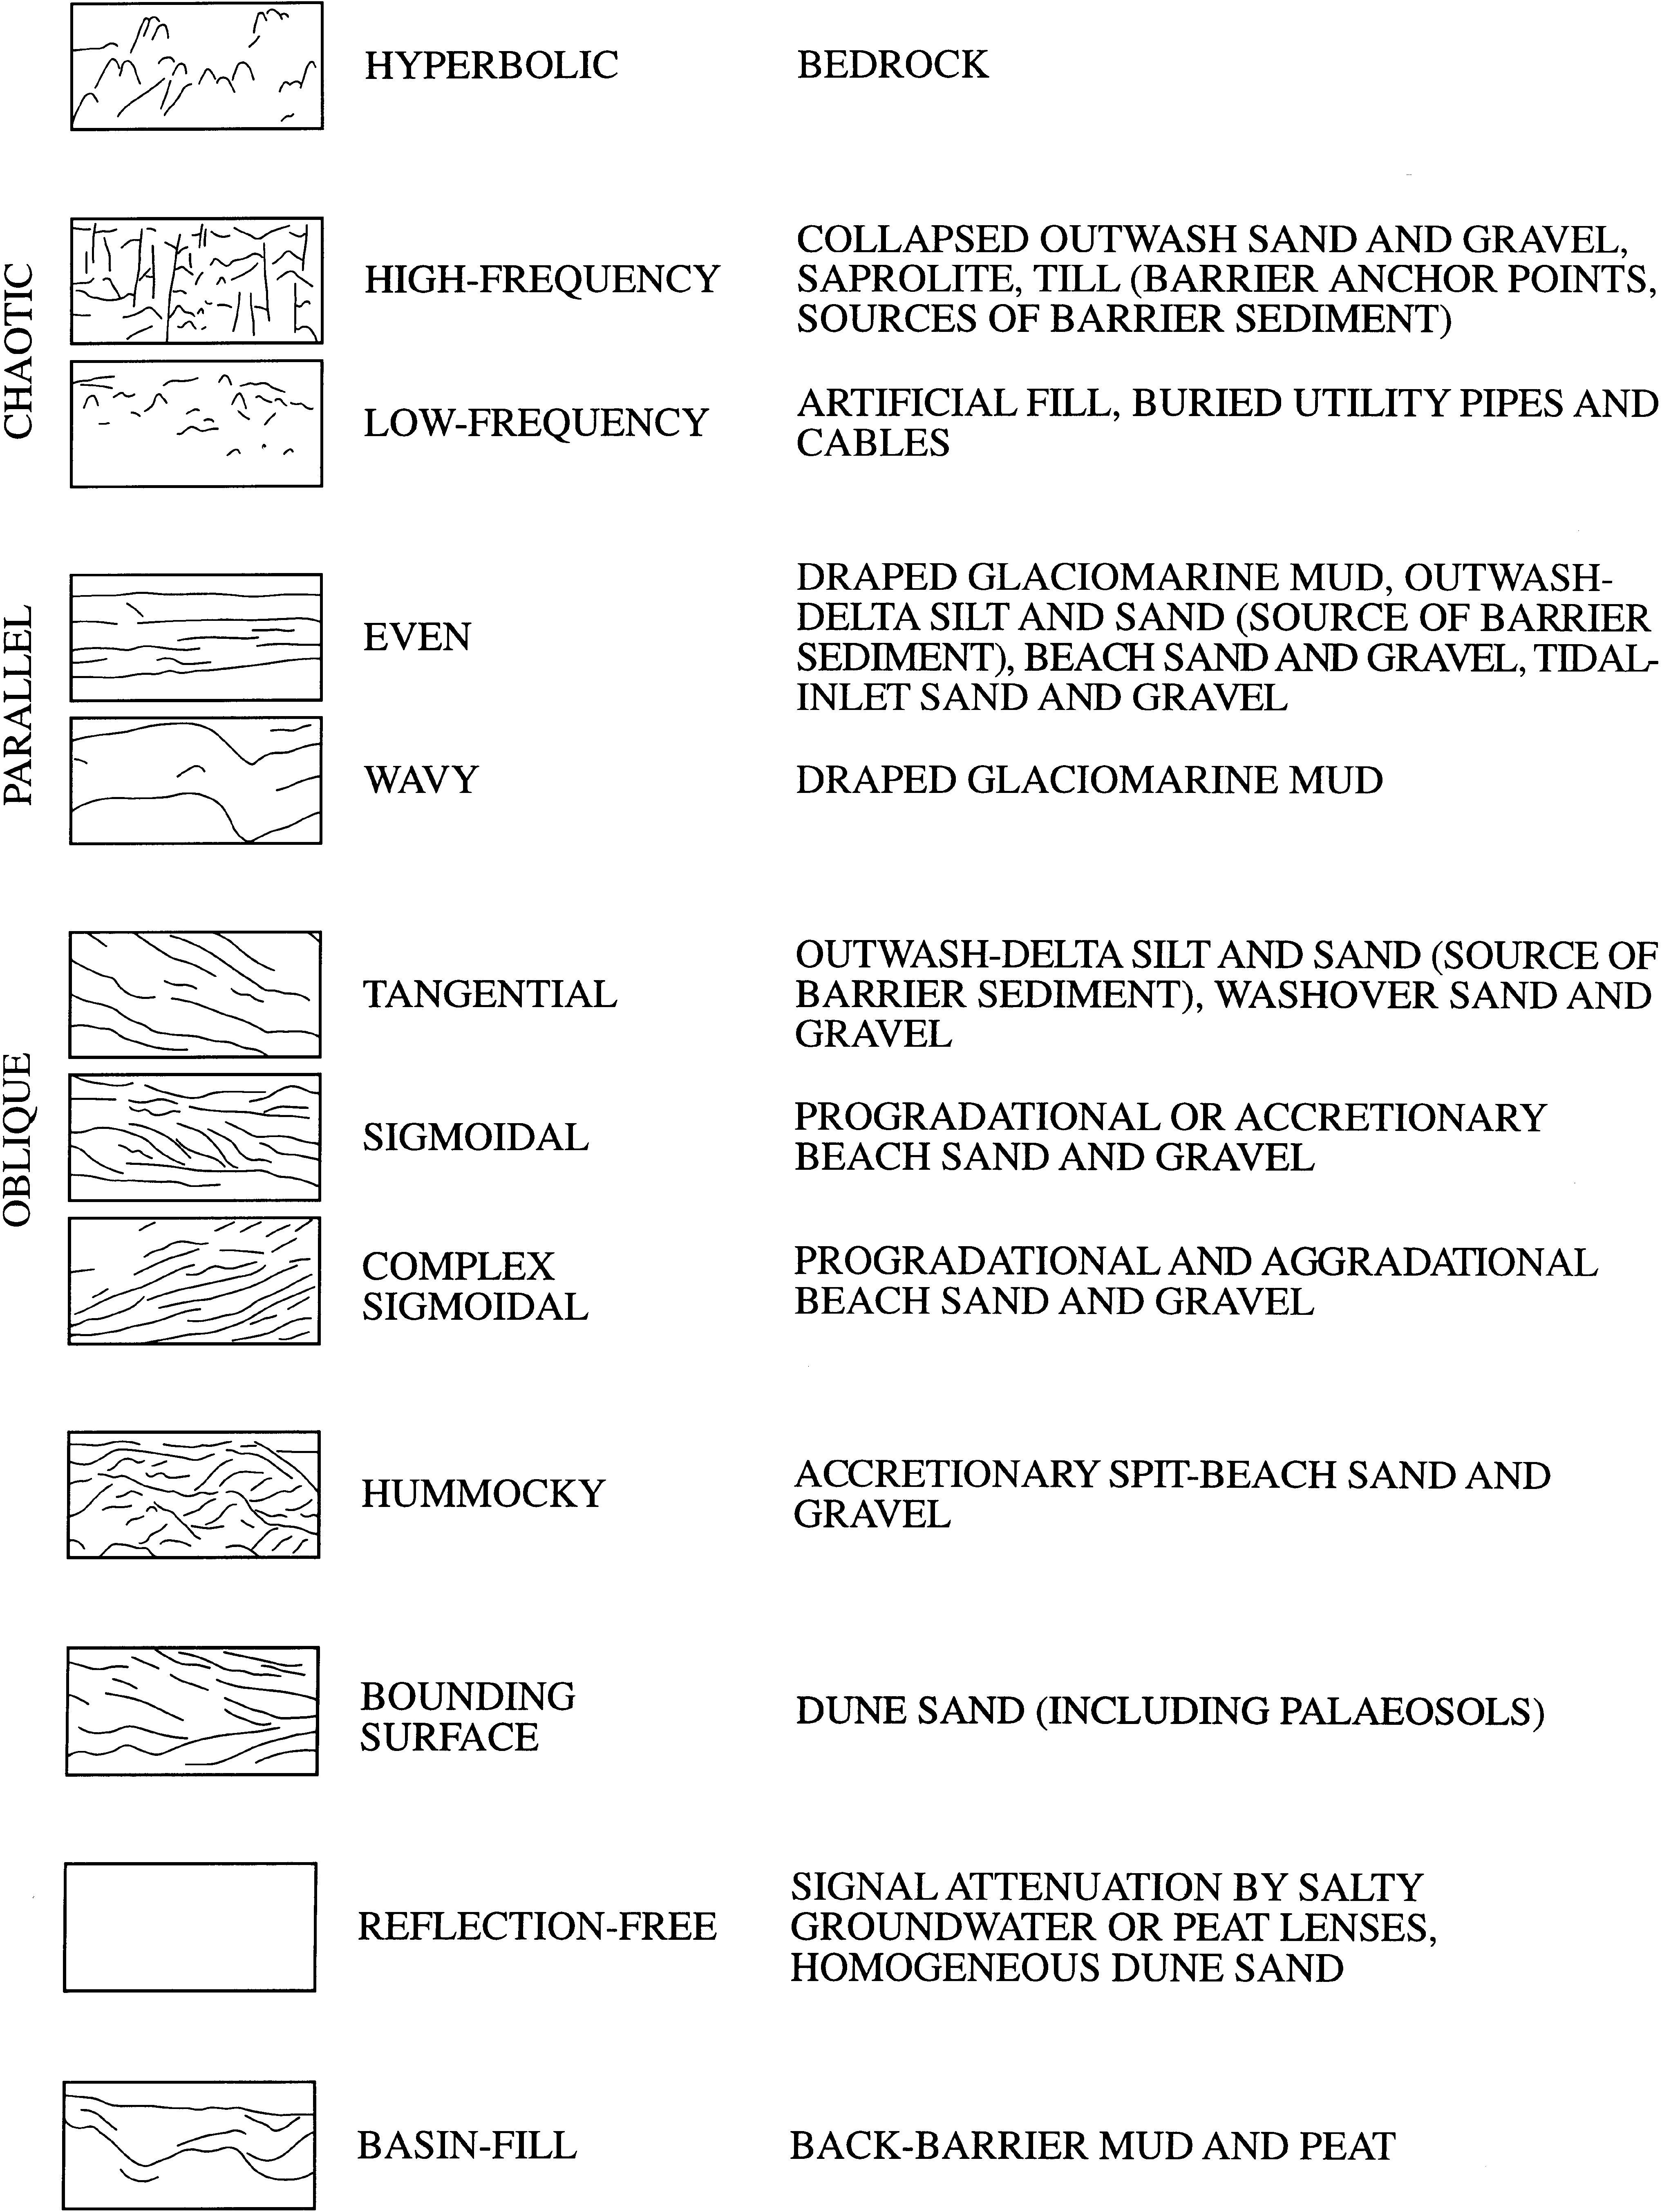
\includegraphics[width=0.9\linewidth]{Figures/0.2GPR/VanHeteren_1998_Coastal.png}
    \caption[Paraglacial coastal setting.]{Paraglacial coastal setting. \textbf{Keywords: } Chaotic, parallel, oblique, hyperbolic, high-frequency, low-frequency, tangential, sigmoidal, hummocky, bounding surface \citep{VanHeteren1998}.}
    \label{fig:VanHeteren1998-1}
\end{figure}